\documentclass[10pt]{article}
\usepackage{icmlko}

\icmlmeta{IP 파운데이션 월드모델}{115}{나침반은 없었다}{노트 114가 지목한 ``같은 관계''를 쟀더니 순환부터 나왔고, 고치자 분리가 사라졌다 --- 라벨 상관 · 잔차에 이어 세 번째 실패다}

\begin{document}

\twocolumn[
\icmlheader

\begin{abstract}
노트 114가 길을 가리켰다 --- 정렬에 필요한 것은 같은 \emph{개념}이 아니라
같은 \emph{관계}다(Meredith 1993의 형태 불변). 그것을 재면 노트 101(라벨
상관)과 104(잔차)가 두 번 실패한 ``긁기 전에 축을 고르는 기준''이 생긴다.
쟀다. 축 $a$ 가 기준 축들과 맺는 상관 벡터를 도메인마다 만들고, 도메인 쌍
사이의 코사인 유사도를 평균해 \textbf{관계 일치도}로 삼았다. \textbf{첫 계산이
완벽해 보였다} --- 채택된 공통 축이 $+$0.50$\sim+$0.97, 긁은 후보 스무 개가
$+$0.40 이하로 \emph{깨끗이} 갈렸다. \textbf{그런데 순환이 있었다.} 기준 축에
자기 자신이 들어가면 $\rho(a,a){=}1$ 이 어느 도메인에서나 같아 일치도가
부풀려진다 --- 매장 노출이 \textbf{$+$0.969에서 $+$0.280으로} 떨어진다.
고치자 \textbf{분리가 사라진다} --- 채택된 다섯이 $+$0.038$\sim+$0.534이고
후보 스무 개가 $-$0.155$\sim+$0.400으로 겹친다. \textbf{가장 중요한 공통
축(타깃 폭)이 $+$0.038로 후보 열둘보다 낮다.} 예측력도 없다 --- 일치도와
잔차의 상관이 $-$0.158, 일치도와 $\Delta$판정치가 $+$0.002다. \textbf{다만
측정 자체는 튼튼하다} --- 반쪽을 건너 $r{=}+$0.525로 재현된다. 잡음이 아니라
진짜 양인데 우리가 원하는 것을 안 맞힌다. \textbf{세 번째 실패다.} 세 가지
그럴듯한 기준이 독립으로 죽었다는 것은 하나를 뜻한다 --- \textbf{어떤 축이
공통 축이 될지는 축 자체의 성질로 결정되지 않는다.} 축과 \emph{나머지 구조
전체}의 상호작용이다. 그러면 남는 길은 하나다 --- 나침반을 찾는 대신
\textbf{검정을 싸게 만든다.}
\end{abstract}
]

\begin{figure*}[t]
\centering
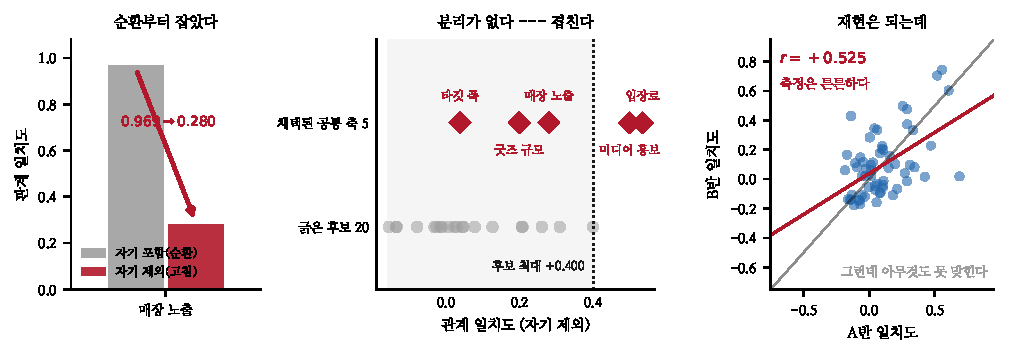
\includegraphics[width=\textwidth]{figs/nc.pdf}
\caption{왼쪽 --- 순환부터 잡았다. 가운데 --- 분리가 없다. 오른쪽 ---
재현은 되는데.}
\end{figure*}

\section{순환부터 잡았다}

관계 일치도의 첫 계산은 이랬다.

\begin{table}[t]
\centering\tsize
\caption{첫 계산 --- 완벽해 보였다.}
\begin{tabular}{lr}
\toprule
매장 노출 & $+$0.969 \\
입장료 & $+$0.534 \\
미디어 홍보 & $+$0.499 \\
\midrule
긁은 후보 스무 개 & $-$0.155 $\sim$ $+$0.400 \\
\bottomrule
\end{tabular}
\end{table}

발표할 뻔했다. 그런데 기준 축 셋에 매장 노출 자신이 들어 있었다 ---
$\rho(a,a){=}1$ 이 모든 도메인에서 같으므로 벡터들이 그 성분을 공유하고
코사인이 부풀려진다. \textbf{자기 자신을 빼니 $+$0.969가 $+$0.280이 된다.}

\claimx{\textbf{순환이 있었다.} 축이 자기 기준에 들어가면 일치도가 인위로
높아진다. 입장료 · 미디어 홍보는 기준 축이 아니라 영향이 없었지만, 그 둘만
보고 ``분리된다''고 했으면 틀렸을 것이다.}{순환을 잡은 것은 채택된 축 셋 중
셋(타깃 폭 · 굿즈 규모 · 매장 노출)뿐이다. 이 셋이 기준이므로 구조상 순환이
생긴다 --- 다른 기준 집합을 쓰면 다른 값이 나온다.}

\section{고치자 분리가 사라졌다}

\begin{table}[t]
\centering\tsize
\caption{자기 자신을 뺀 관계 일치도.}
\begin{tabular}{lrrr}
\toprule
& 일치도 & 도메인 & 잔차 \\
\midrule
\multicolumn{4}{l}{\emph{채택된 공통 축 다섯}} \\
입장료 & $+$0.534 & 8 & 1.326 \\
미디어 홍보 & $+$0.499 & 4 & 0.451 \\
매장 노출 & $+$0.280 & 8 & 0.814 \\
굿즈 규모 & $+$0.199 & 8 & 0.604 \\
\textbf{타깃 폭} & \textbf{$+$0.038} & 8 & \textbf{0.620} \\
\midrule
\multicolumn{4}{l}{\emph{긁은 후보 스무 개}} \\
표지 주성분 & $+$0.400 & 7 & 1.207 \\
설명문 문장 수 & $+$0.310 & 7 & 1.150 \\
$\cdots$ 중앙값 & $+$0.026 & & \\
최소 & $-$0.155 & & \\
\bottomrule
\end{tabular}
\end{table}

\claimx{\textbf{분리가 없다.} 채택된 다섯이 $+$0.038$\sim+$0.534, 후보 스무
개가 $-$0.155$\sim+$0.400으로 겹친다. \textbf{가장 중요한 공통 축인 타깃 폭이
$+$0.038로 후보 스무 개 중 열둘보다 낮다} --- 그런데 잔차는 0.620으로 가장
좋은 축 축에 든다.}{도메인 수가 다르다(미디어 홍보 4, 나머지 7--8). 적은
도메인의 일치도는 쌍이 적어 흔들린다.}

\begin{table}[t]
\centering\tsize
\caption{예측력.}
\begin{tabular}{lr}
\toprule
일치도 vs 정렬 잔차 & $r{=}-$0.158 \\
일치도 vs $\Delta$판정치 & $r{=}+$0.002 \\
잔차 vs $\Delta$판정치 & $r{=}+$0.008 \\
\bottomrule
\end{tabular}
\end{table}

\section{재현은 되는데 쓸모가 없다}

일치도가 잡음이라 실패했다면 이야기가 간단하다. \textbf{아니다.}

\claimx{관계 일치도는 \textbf{튼튼한 측정}이다 --- 레코드를 반으로 갈라 각
반쪽에서 다시 재면 $r{=}+$0.525로 맞는다(칸 60개, 분할 셋). 잡음이 아니라
진짜 양이다. \textbf{그런데 우리가 원하는 것을 안 맞힌다.}}{$+$0.525 가
아주 높지는 않다. 반쪽에서는 도메인마다 레코드가 절반이라 상관 추정이
흔들린다.}

\section{세 번째 실패}

\begin{table}[t]
\centering\tsize
\caption{``긁기 전에 축을 고르는 기준''의 시도.}
\begin{tabular}{lll}
\toprule
& 기준 & 죽은 방식 \\
\midrule
노트 101 & 라벨 상관 & 노트 102 --- 반쪽 검정에서 \\
& & 무작위보다 못했다 \\
노트 104 & 정렬 잔차 & 방향이 반대였다 \\
& & (잘 맞으면 중복) \\
\textbf{노트 115} & \textbf{관계 일치도} & \textbf{분리가 없다} \\
\bottomrule
\end{tabular}
\end{table}

\claimx{세 가지 그럴듯한 기준이 독립으로 죽었다. \textbf{어떤 축이 공통 축이
될지는 축 자체의 성질로 결정되지 않는다} --- 축과 \emph{나머지 구조 전체}의
상호작용이다. 같은 축도 다른 공통 축 집합 아래서는 다르게 행동한다(노트 103 ·
105 · 108이 그것을 세 번 보였다).}{세 기준이 전부 ``축 하나를 보는'' 것이었다.
축 \emph{쌍}이나 축 \emph{집합}의 성질을 보는 기준은 안 시도했다.}

\begin{quote}\fontsize{9.5}{11.5}\selectfont
\textbf{그러면 남는 길은 하나다 --- 나침반을 찾는 대신 검정을 싸게 만든다.}
지금 씨앗 넷 짝지은 붓스트랩 한 번이 5$\sim$10분이다. 후보 스무 개를 다
판정하면 서너 시간이다. \textbf{그것을 몇 분으로 줄이면 나침반이 필요 없다.}
\end{quote}

\section{한계}

\begin{itemize}[leftmargin=1.1em,itemsep=0.15em]
\item 기준 축을 채택된 공통 축 셋으로 잡았다. 다른 기준 집합이면 일치도가
      달라진다 --- 순환을 완전히 못 없앤다.
\item 후보가 스무 개뿐이고 전부 설명문 · 표지에서 나왔다.
\item 일치도를 상관 벡터의 코사인으로 정의했다. 다른 정의(부분 상관 · 회귀
      계수)는 안 해 봤다.
\item 반쪽 재현 $r{=}+$0.525 가 아주 높지 않다.
\item 축 쌍 · 축 집합의 성질을 보는 기준은 안 시도했다.
\end{itemize}

\section{다음}

\begin{enumerate}[leftmargin=1.3em,itemsep=0.15em]
\item \textbf{검정을 싸게 만든다} --- 나침반 찾기를 접고 판정 속도를 올린다.
      지금 병목은 붓스트랩 반복마다 인자 공간을 다시 만드는 것이다. 적재만
      바뀌는 설정은 다시 안 만들어도 된다. \textbf{목표는 후보 하나당 1분.}
\item \textbf{팝업 레코드} --- 아홉 노트가 같은 곳을 가리킨다.
\item 텀블벅 API --- 펀딩만 미디어 홍보 0\%다.
\item 축 \emph{집합}의 성질 --- 하나씩 보는 기준이 셋 다 죽었으니 다음은
      집합이다.
\end{enumerate}

\vspace{0.6em}
\hrule height 0.3pt
\vspace{0.5em}
{\footnotesize
\textbf{참고문헌}\\[0.3em]
Meredith, W. (1993). Measurement invariance, factor analysis and factorial
invariance. \emph{Psychometrika}, 58(4), 525--543.\\[0.15em]
Guyon, I., Elisseeff, A. (2003). An introduction to variable and feature
selection. \emph{JMLR}, 3, 1157--1182.\\[0.15em]
Schoenemann, P. H. (1966). A generalized solution of the orthogonal Procrustes
problem. \emph{Psychometrika}, 31(1), 1--10.\\[0.15em]
Cawley, G. C., Talbot, N. L. C. (2010). On over-fitting in model selection and
subsequent selection bias in performance evaluation. \emph{JMLR}, 11, 2079--2107.\\[0.15em]
Ben-David, S. et al. (2010). A theory of learning from different domains.
\emph{Machine Learning}, 79(1--2), 151--175.
}

\end{document}
